\textbf{/F30/} \\
\textbf{Prozess:} Mitglieder in eine Gruppe einladen\\
\textbf{Ziel:} Mitglieder erhalten einen Link zur Gruppe\\
\textbf{Kategorie:} primär\\
\textbf{Vorbedingung:} Gruppe wurde bereits erstellt\\
\textbf{Nachbedingung} (Erfolg): zukünftige Gruppenmitglieder erhalten einen Link\\
\textbf{Nachbedingung} (Fehlschlag): zukünftige Gruppenmitglieder erhalten keinen Link\\
\textbf{Akteure:} Gruppenadministrator\\
\textbf{Auslösendes Ereignis:} Ein oder mehrere Personen sind noch nicht Mitglieder der Gruppe\\
\textbf{Beschreibung:}\\
1.) Gruppenadministrator macht sich Gedanken welche Personen er in die Gruppe einladen möchte\\
2.) Er tippt auf den Namen der Gruppe und sieht die allgemeinen Informationen über die Gruppe (Namen, Mitglieder)\\
3.) Über "Share Link" kann er auswählen, über welchen externen Messenger er den Link weiterleiten möchte\\
4.) Er wählt den gewünschten Messenger und seine Kontakte und bestätigt\\
5.) Link wird an die ausgewählten Kontakte versendet\\
\\

\begin{figure} [H]
	\centering
	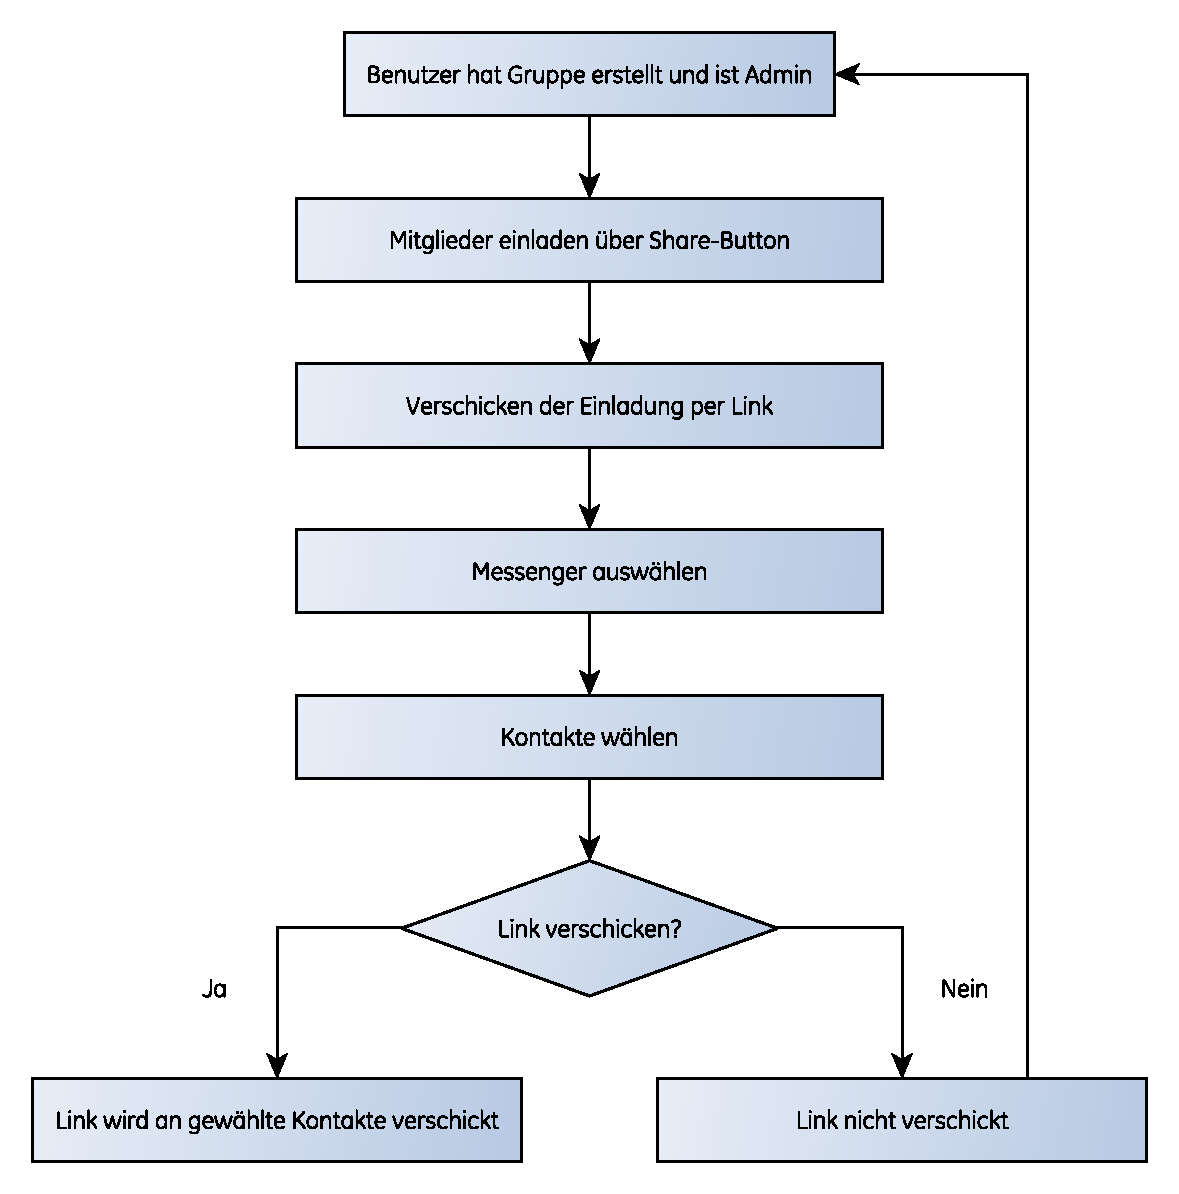
\includegraphics[scale=0.7]{./res/F30_mitglieder_einladen_flowgraph.pdf}
\end{figure}

